% тут сначала про данные и задачу, плюс много слов о том, почему это валидная задача
% потом таблички?? это в теории должна быть самая мясная часть работы и хорошо бы уже иметь хоть половину её написанной к пред защите, которая блин уже во вторник(((
% 
\chapter{Experiments and results}

% (сюда можно дописать еще общих слов из \cite{beyer2020_are_we_done}) для объема

This section presents the results of the experiments conducted. The modifications described in \autoref{chap:speed} and \autoref{chap:performance} are applied one-by-one to better understand impact of each refinement. The models are evaluated on standard Imagenet training with input resolution fixed to 224, their top-1 accuracy and GPU throughput is compared to other known models such as EfficientNet \cite{tan2019_efficientnet}. The baseline ResNet50 gets 76.7\% top-1 accuracy on our codebase which is on par with original results of 76.5\%. We improve its performance up to 79.6\% (\textcolor{blue}{+3.1\%}) by \textit{better training methods alone}. By adding several common and simple changes in architecture (Anti-Alias downsampling, Efficient Channel Attention, Improved Stem and Swish activation) the performance could be further boosted up to 81.0\%. We demonstrate that majority of the improvement comes from training methods rather than architecture modifications, despite training methods often perceived as a less important factor for CNNs.  

\autoref{tab:resnet_method_ablation} presents an additive study of training, augmentation/regularization and architectural changes. We find it's important to reduce the weight decay factor after a sufficient number of regularization methods have been added, in order to avoid over-regularizing the network. Smaller weight decay values have been used in other works \cite{tan2019_efficientnet} \cite{bello2021_revisiting_resnet} but they didn't point out the importance of it in presence of extra regularization. Due to limited resources, we didn't perform an ablation study for best weight decay, reducing it to 2e-5 worked well in our experiments.

\newcommand{\improvement}[1]{\textcolor{blue}{#1}}
\newcommand{\decrease}[1]{\textcolor{red}{#1}}
\newcommand{\improvementb}[1]{\textbf{#1}}
% \newcommand{\improvementb}[1]{\textcolor{green}{\textbf{#1}}}
\newcommand{\decreaseb}[1]{#1}
% TODO: ask Dja what looks better, maybe don't add inference speed to first blue and green rows
\begin{table}[ht!]
    \begin{center}
    \small
    \begin{tabular}{l|cc|c}
      \toprule
      Improvements & Top-1 & $\Delta$  & Inference Speed\\
      \hline
      \hline
      ResNet-50 & 76.7 & --- & 2630\\
      \rowcolor{blue!15}
      + Tune Learning Rate schedule: Stepwise $\rightarrow$ Cosine & 77.0 & \improvementb{+0.3} & 2630\\
      \rowcolor{blue!15}
      + Change Optimizer: SGD $\rightarrow$ RMSProp & 77.2 & \improvementb{+0.2} & 2630\\
      \rowcolor{blue!15}
      + Longer training: 90 epochs $\rightarrow$ 240 epochs& $\;\;$76.4 $^\dag$ & \decreaseb{-0.8} & 2630 \\
      % \hdashline
      \rowcolor{green!20}
      + Stronger augmentations: RandAug + CutMix & 77.6 & \improvementb{+1.2} & 2630\\
      \rowcolor{green!20}
      + Label Smoothing & 77.9 & \improvementb{+0.3} & 2630\\
      \rowcolor{green!20}
      + Stochastic Depth & 78.1 & \improvementb{+0.2} & 2630\\
      \rowcolor{green!20}
      + EMA of weight & 78.3 & \improvementb{+0.2} & 2630\\
      \rowcolor{green!20}
      + Dropout on FC & $\;\;$ 78.2 $^\dagger$ & \decreaseb{-0.1} & 2630\\
      \rowcolor{green!20}
      + Decrease weight decay: 1e-4 $\rightarrow$ 2e-5 & 79.6 & \improvementb{+1.3} & 2630\\
      % \hdashline
      \rowcolor{yellow!20}
      + Anti-Alias Downsampling & 79.8 & \improvementb{+0.2} & 2540 \\
      \rowcolor{yellow!20}
      + Efficient Channel Attention & 80.5 & \improvementb{+0.7} & 2235 \\
      \rowcolor{yellow!20}
      + Better activation: ReLU $\rightarrow$ Swish & 80.9 & \improvementb{+0.4} & 2120 \\
      \rowcolor{yellow!20}
      + SpaceToDepth Stem & 81.0 & \improvementb{+0.1} & 2250 \\
      % \rowcolor{yellow!20}
      % + Different Block Selection & 81.3 & \improvementb{+0.1} & ??? \\
      \bottomrule
    \end{tabular}
    \end{center}
    \vspace{-0.15cm}
    \caption{\textbf{Additive study of the ResNet-50 training improvements.} The colors in the table refer to \textbf{\colorbox{blue!15}{Training Methods}}, \textbf{\colorbox{green!20}{Regularization / Augmentaion Refinements}} and \textbf{\colorbox{yellow!20}{Architecture Changes}}. See Section \ref{subsec: baseline_training} for details baseline ResNet-50 training. The image resolution for all experiments was kept fixed at $224 \times 224$. Top-1 accuracy is measured on the Imagenet \texttt{validation-set}. $^{\dag}$ The drop is due to over-fitting. Longer training only becomes useful after adding more regularization. $^{\ddagger}$ Dropout on FC leads to over regularization of the model. Improvement from this step are beneficial only after reducing weight decay.
    %(See Table~\ref{tab:wd_analysis} for more details). I don't have this table and probably wouldn't have time for it. Leave just as a possible thing to do in the future. (lol what future). TODO: 
    }
    \label{tab:resnet_method_ablation}
    \end{table}

% speed measurements for models. To have a reference. Conclusion from this: 
% AA makes it ~8% slower. but if we only use AA on main path it's 3.5% slowdown
% ECA slowdowns by ~12% 
% Space2Depth + 5% (because we measure with 4x4 s2d. it's cheating but nobody cares)

% Initialized models
% R50 25.56M params
% Mean of 5 runs 10 iters each BS=256, SZ=224:
%           97.22+-0.04 msecs Forward. 0.00+-0.00 msecs Backward. Max memory: 1987.86Mb. 2633.10 imgs/sec
% R50-D AA 25.56M params
% Mean of 5 runs 10 iters each BS=256, SZ=224:
%           105.61+-0.04 msecs Forward. 0.00+-0.00 msecs Backward. Max memory: 2038.86Mb. 2424.10 imgs/sec
% R50-D AA + ECA 25.56M params
% Mean of 5 runs 10 iters each BS=256, SZ=224:
%           119.27+-0.03 msecs Forward. 0.00+-0.00 msecs Backward. Max memory: 2089.75Mb. 2146.42 imgs/sec
% R50-D AA + ECA + S2D 25.58M params
% Mean of 5 runs 10 iters each BS=256, SZ=224:
%           112.64+-0.04 msecs Forward. 0.00+-0.00 msecs Backward. Max memory: 2139.52Mb. 2272.76 imgs/sec
% R50-D AA + ECA + S2D + swish 25.58M params
% Mean of 5 runs 10 iters each BS=256, SZ=224:
%          128.36+-0.03 msecs Forward. 0.00+-0.00 msecs Backward. Max memory: 2038.96Mb. 1994.40 imgs/sec
% R50-D AA + ECA + S2D + swish hard 25.58M params
% Mean of 5 runs 10 iters each BS=256, SZ=224:
%          126.52+-0.05 msecs Forward. 0.00+-0.00 msecs Backward. Max memory: 2089.89Mb. 2023.43 imgs/sec

\section{Setup}
All training was performed on 4 x Tesla V100 GPUs with batch size 256 per device (1024 in total for most experiments). We used linear learning rate warm-up for the first 5 epochs. The base learning rate was fixed at 0.1 per 256 batch (0.4 in our experiments with 1024 batch size) for SGD and 0.016 for RMSProp optimizer (0.064 in our experiments with 1024 batch size). We use momentum in optimizer 0.9, batch norm momentum 0.99. For exponential moving average we use momentum 0.9995 inspired by \cite{tan2021_efficientnetv2}. For Cutmix we set alpha to 0.1. Dropout on the last Fully Connected layer is increased from 0 at the beginning of the training to 0.2 at 50-th epoch. Survival probability in Drop Block is linearly decreased each network block from 1 to 0.8. For Label Smoothing, we use a smoothing value of 0.1. Following tricks described in \autoref{sec: large-batch} we only applied weight decay to weights of convolutional and linear layers and initialized $\gamma$ for last BN in each block to 0. All code was written on PyTorch v1.8.1 and is available on \href{https://github.com/bonlime/sota_imagenet/}{GitHub}

\section{Architecture changes}
We call the best model from \autoref{tab:resnet_method_ablation} as ResNet50-AA-ECA-S2D. Visualization of it's architecture could be seen on \autoref{fig:resnet-aa-eca-s2d}. This model incorporates all suggested modifications mentioned in \autoref{chap:performance} into one network, to explore the additive effect of each of them.   


\begin{figure}[h!]
    \centering
    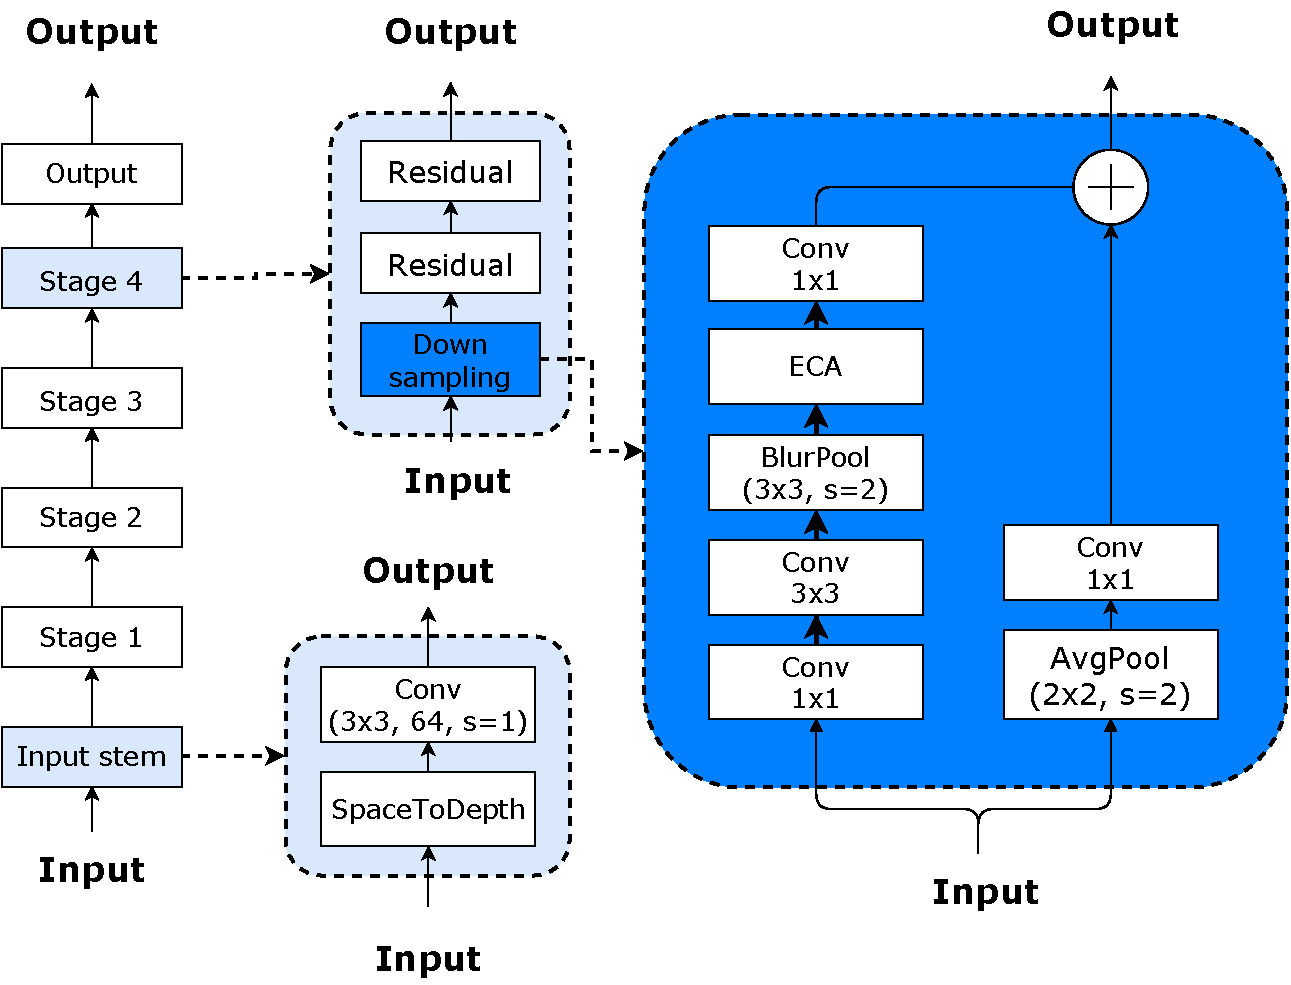
\includegraphics[width=0.8\textwidth]{images/full_network.pdf}
    \caption{Architecture of proposed ResNet50-AA-ECA-S2D model.}
    \label{fig:resnet-aa-eca-s2d}
  \end{figure}


\begin{figure}[h!]
    \centering
    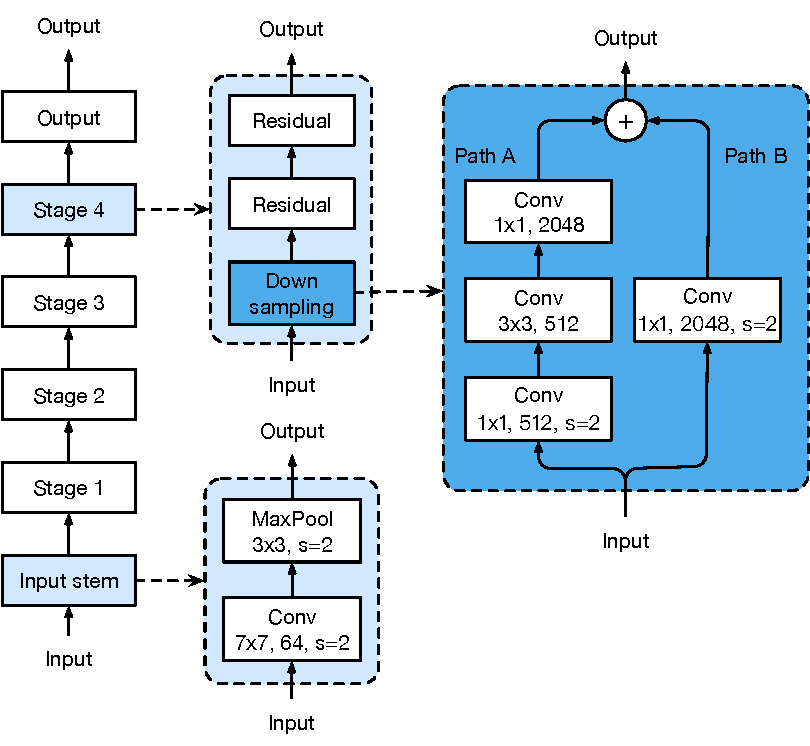
\includegraphics[width=0.8\textwidth]{images/resnet-a.pdf}
    \caption{Architecture of default ResNet-50.}
    \label{fig:resnet-a_2}
  \end{figure}

% RMSProp optimizer with decay 0.9 and
% momentum 0.9; batch norm momentum 0.99; weight decay 1e-5. Each model is trained for 350 epochs with a total
% batch size of 4096. Learning rate is first warmed up from 0
% to 0.256, and then decayed by 0.97 every 2.4 epochs. We
% use exponential moving average with 0.9999 decay rate,
% RandAugment (Cubuk et al., 2020), Mixup (Zhang et al.,
% 2018), Dropout (Srivastava et al., 2014), and stochastic
% depth (Huang et al., 2016) with 0.8 survival probability


% First we validate out setup by re-training original ResNet50 and ResNet34 model from \cite{he2016deep_resnetv1} paper. 



% experiment numbers from Bag of Tricks
% Heuristic BS=256 BS=1024
% Top-1 Top-5 Top-1 Top-5
% Linear scaling 75.87 92.70 75.17 92.54
% + LR warm-up 76.03 92.81 75.93 92.84
% + Zero γ 76.19 93.03 76.37 92.96
% + No bias decay 76.16 92.97 76.03 92.86
% + FP16 76.15 93.09 76.21 92.97


% add a note that while an order of applying changes does matter it doesn't affect the final results. Maybe also add a note that no real conclusions about most effective regularization and training tricks could be done because it's always order dependant. Making a legit comparison is impossible due to the computation cost of Imagenet training and an overwhelming amount of possible variations. 


\section{Ablation study} \label{sec:ablation}

This section presents the results of ablation studies, which were performed in order to validate the little design choices of the final model. 

\subsection{Channel Attention}
We tested two variants of Channel Attention described in \autoref{sec:channel-attn}: Squeeze-Excitation (SE) and Efficient Channel Attention (ECA). In both cases, attention is introduced after the $3 \times 3$ convolution in the Bottleneck block. As could be seen from results in \autoref{table:se_vs_eca} ECA clearly outperforms SE both in top-1 accuracy and in inference speed. It also introduces only a negligible amount of new parameters which is beneficial as it helps to reduce overfitting. The inference speed of SE and ECA variants is very close, despite the former having a much smaller number of FLOPs. It happens because of the Global Average Pooling (GAP) operation present in both types of attention, which is responsible for most of the slowdown. The models for this ablation are trained for 90 epochs using the default Imagenet procedure as described in \autoref{subsec: baseline_training}
% TODO: resnet SE + ECA

\begin{table}[h!]
    \centering
    \begin{tabular}{|p{2.9cm}|p{2.7cm}|p{2cm}|p{2.8cm}|p{2.5cm}|}
    \hline
    Models & Top-1 Accuracy & Params (M) & Inference Speed {[}imgs/sec{]} & Training speed {[}imgs/sec{]} \\ \hline
    ResNet50       & 76.61          & 25.56 & \textbf{2630} & 492 \\ 
    ResNet50 + SE  & 77.52          & 28.09 & 2280          & 438 \\ 
    ResNet50 + ECA & \textbf{77.62} & 25.56 & 2320          & 436 \\ \hline
    \end{tabular}
    \caption{Comparsion of different channel attentions}
    \label{table:se_vs_eca}
    \end{table}


% Initialized models
% R50 25.56M params
% Mean of 5 runs 10 iters each BS=256, SZ=224:
% 	 131.27+-0.08 msecs Forward. 388.78+-3.92 msecs Backward. Max memory: 10936.48Mb. 492.26 imgs/sec
% R50 SE 28.09M params
% Mean of 5 runs 10 iters each BS=256, SZ=224:
% 	 146.15+-0.04 msecs Forward. 438.22+-2.55 msecs Backward. Max memory: 13771.25Mb. 438.08 imgs/sec
% R50 ECA 25.56M params
% Mean of 5 runs 10 iters each BS=256, SZ=224:
% 	 145.03+-0.05 msecs Forward. 441.98+-2.51 msecs Backward. Max memory: 13863.32Mb. 436.11 imgs/sec

% Initialized models
% R50 25.56M params
% Mean of 5 runs 10 iters each BS=256, SZ=224:
% 	 97.41+-0.01 msecs Forward. 0.00+-0.00 msecs Backward. Max memory: 1987.86Mb. 2628.01 imgs/sec
% R50 SE 28.09M params
% Mean of 5 runs 10 iters each BS=256, SZ=224:
% 	 112.30+-0.02 msecs Forward. 0.00+-0.00 msecs Backward. Max memory: 2043.68Mb. 2279.56 imgs/sec
% R50 ECA 25.56M params
% Mean of 5 runs 10 iters each BS=256, SZ=224:
% 	 110.66+-0.02 msecs Forward. 0.00+-0.00 msecs Backward. Max memory: 2094.55Mb. 2313.35 imgs/sec

% Ablation ECA vs SE
% exp 108, 110, 111
% R50 + HardReg
% [01-11 17:22:04] - Val   loss: 1.8560 | Acc@1: 76.6160 | Acc@5: 93.3100
% R50 + HardReg + SE
% [01-11 23:51:53] - Val   loss: 1.8135 | Acc@1: 77.5260 | Acc@5: 93.7700
% R50 + HardReg + ECA
% [01-13 14:56:35] - Val   loss: 1.7983 | Acc@1: 77.6180 | Acc@5: 93.9180
% ECA is slightly faster + have 3M less params but is still better. Pure win-win

\subsection{Input stem} \label{subsec:stem_ablation}

In neural networks the first couple of layers are usually called "stem" layers, their goal is to quickly reduce the resolution of the input image. The stem layer of ResNet50 is compromised of $7 \times 7$ convolution with stride 2, followed by max-pooling with stride 2 \cite{he2016deep_resnetv1}, together these layers decrease input resolution by a factor of 4, after that the first stage of ResNet doesn't reduce the resolution. We explored two possible alternatives for the default input stem. First is ResNet50-D which replaces $7 \times 7$ Conv with three $3 \times 3$ layers, the idea is to achieve the same receptive field by using a lower number of parameters. This does increase performance but gives a slowdown due to multiple $3 \times 3$ convolutions being slower than one $7 \times 7$ expensive convolution and having 3x number of FLOPs. The second design choice is to use the SpaceToDepth module described in \autoref{subsec:space2depth} to reduce resolution 2x, follow by simple convolution to match the number of input channels of the first block. Additionally, we need to change stride of the first stage of ResNet to perform the second reduction in resolution. The proposed variants are illustrated in \autoref{fig:resnet-aa-eca-s2d}.
And their performance comparisons are presented in \autoref{table:stem_comparison}. The expected improvement in GPU throughput could be clearly seen for the space2depth model, the fact that performance also improves slightly is somewhat surprising. One possible explanation could be that aggressive downsampling in the default stem leads to "information loss" - details from the input image are not propagated properly and some of them are lost. SpaceToDepth has almost the same receptive field ($6 \times 6$) as the default stem ($ 7 \times 7$), but is both faster and gives better accuracy. So we choose it as a default stem for all our experiments.

% number of FLOPs
% default stem: 112 x 112 x (3 x 64 x 7 x 7) = 112^2 * 9408
% ResNet-D stem: 112 x 112 x (3 x 32 x 3 x 3) + 112 x 112 (32 x 32 x 3 x 3) + 112 x 112 (32 x 64 x 3 x 3) = 112^2 * 28500

% number of params
% default: 3 x 64 x 7 x 7 = 9400
% resnetD: 3 x 3 x (3 x 32 + 32 x 32 + 32 x 64) = 28500
% s2d: 7000

% another copy-paste from TResNet
% SpaceToDepth: The SpaceToDepth module provides improvements to all the indices. Notice that while we are not the first to use this innovative module (see [33]), we are the first to integrate it into a high-performance network as a drop-in replacement for the traditional convolution-based stem, and get a meaningful improvement. While the GPU throughput improvement is expected, the fact that also the accuracy improves (marginally) when replacing the ResNet stem cell with a ”cheaper” SpaceToDepth unit is somewhat surprising. This result supports our intuition that there could be ”information loss” within the convolution-based stem unit - details from the original image are not propagated well due to the aggressive downscaling process. Although simpler, a SpaceToDepth module minimizes this loss and enables to process of the data via the residual blocks, which are protected from information loss by the skip connections. We will further investigate this issue in future works

% below is copy-paste from TResNet paper
% SpaceToDepth Stem - Neural networks usually start with a stem unit - a component whose goal is to quickly reduce the input resolution. ResNet50 stem is comprised of a stride-2 conv7x7 followed by a max-pooling layer [10], which reduces the input resolution by a factor of 4 (224 → 56). ResNet50-D stem design [11], for comparison, is more elaborate - the conv7x7 is replaced by three conv3x3 layers. The new ResNet50-D stem design did improve accuracy, but at a cost of lowering the training throughput - see Table 1, where the new stem design is responsible for almost all the decline in the throughput. We wanted to replace the traditional convolution-based downscaling unit with a fast and seamless layer, with as little information loss as possible, and let the well-designed residual blocks do all the actual processing work. The new stem layer sole functionality should be to downscale the input resolution to match the rest of the architecture, e.g., by a factor of 4. We met these goals by using a dedicated SpaceToDepth transformation layer [33], that rearranges blocks of spatial data into depth. Notice that in contrast to [33], which mainly used SpaceToDepth in the context of isometric (single-resolution) networks, in our novel design SpaceToDepth is used as a drop-in replacement for the traditional stem unit. The SpaceToDepth layer is followed by simple convolution, to match the number of wanted channels, as can be seen in Figure 1.

% there are no real experiments with R50 + s2d. there are only experiments with an already modified R34-50 network. But
% in order not to confuse the reader I'll say it's R50
% [08-12 04:28:27] - Acc@1 75.122 Acc@5 92.352
% [08-12 08:02:56] - Acc@1 75.514 Acc@5 92.624    

% Initialized models
% R50 25.56M params
% Mean of 5 runs 10 iters each BS=256, SZ=224: ~380us forward
% 	 97.39+-0.01 msecs Forward. 0.00+-0.00 msecs Backward. Max memory: 1987.86Mb. 2628.71 imgs/sec
% R50 s2d 25.58M params
% Mean of 5 runs 10 iters each BS=256, SZ=224: ~350us forward
% 	 90.61+-0.03 msecs Forward. 0.00+-0.00 msecs Backward. Max memory: 2038.88Mb. 2825.16 imgs/sec
% R50 s2d_2 25.59M params
% Mean of 5 runs 10 iters each BS=256, SZ=224:
% 	 93.57+-0.11 msecs Forward. 0.00+-0.00 msecs Backward. Max memory: 2089.81Mb. 2735.78 imgs/sec

% single layer benchmarking. FP16 + BS=128 + torch.cuda.benchmark=True
% 16 threads: --------------------------------
%       conv7x7                 |      18.6
%       conv2x2                 |       3.7
%       conv3x3                 |       5.2
%       space2depth             |      10.4
%       space2depth_jit         |      10.4
%       conv7x7 maxpool (OS=4)  |      23.5
%       space2depth 2x2         |       1.4
%       conv3x3 like in s2d     |       9.0
% Times are in microseconds (us).
% conclusions from this table are: s2p is 2x times faster with the same respective field

% TODO: make table centered
\begin{table}[h!]
    \centering
    \begin{tabular}{|p{3.1cm}|p{2.7cm}|p{2cm}|p{2.8cm}|p{2cm}|}
    \hline
    Models & Top-1 Accuracy & Params (M) & Inference Speed {[}imgs/sec{]} \\ \hline
    ResNet50         & 76.61 & 25.56 & 2630 \\ 
    ResNet50-D Stem  & 76.87 & 25.58 & 2440 \\ 
    ResNet50 + s2d   & \textbf{76.95} & 25.59 & \textbf{2825} \\ \hline
    \end{tabular}
    \caption{Comparison of different input stems.}
    \label{table:stem_comparison}
    \end{table}

% TODO: ablation of ECA vs SE
% TODO: ablation of ECA after conv1x1 vs after conv3x3
% TODO: ablation of Cosine